\documentclass[10pt,a4paper,onecolumn]{article}
\usepackage{marginnote}
\usepackage{graphicx}
\usepackage{xcolor}
\usepackage{authblk,etoolbox}
\usepackage{titlesec}
\usepackage{calc}
\usepackage{tikz}
\usepackage{hyperref}
\hypersetup{colorlinks,breaklinks,
            urlcolor=[rgb]{0.0, 0.5, 1.0},
            linkcolor=[rgb]{0.0, 0.5, 1.0}}
\usepackage{caption}
\usepackage{tcolorbox}
\usepackage{amssymb,amsmath}
\usepackage{ifxetex,ifluatex}
\usepackage{seqsplit}
\usepackage{fixltx2e} % provides \textsubscript
\usepackage[
  backend=biber,
%  style=alphabetic,
%  citestyle=numeric
]{biblatex}
\bibliography{paper.bib}



% --- Page layout -------------------------------------------------------------
\usepackage[top=3.5cm, bottom=3cm, right=1.5cm, left=1.0cm,
            headheight=2.2cm, reversemp, includemp, marginparwidth=4.5cm]{geometry}

% --- Default font ------------------------------------------------------------
% \renewcommand\familydefault{\sfdefault}

% --- Style -------------------------------------------------------------------
\renewcommand{\bibfont}{\small \sffamily}
\renewcommand{\captionfont}{\small\sffamily}
\renewcommand{\captionlabelfont}{\bfseries}

% --- Section/SubSection/SubSubSection ----------------------------------------
\titleformat{\section}
  {\normalfont\sffamily\Large\bfseries}
  {}{0pt}{}
\titleformat{\subsection}
  {\normalfont\sffamily\large\bfseries}
  {}{0pt}{}
\titleformat{\subsubsection}
  {\normalfont\sffamily\bfseries}
  {}{0pt}{}
\titleformat*{\paragraph}
  {\sffamily\normalsize}


% --- Header / Footer ---------------------------------------------------------
\usepackage{fancyhdr}
\pagestyle{fancy}
\fancyhf{}
%\renewcommand{\headrulewidth}{0.50pt}
\renewcommand{\headrulewidth}{0pt}
\fancyhead[L]{\hspace{-0.75cm}\includegraphics[width=5.5cm]{logo.png}}
\fancyhead[C]{}
\fancyhead[R]{}
\renewcommand{\footrulewidth}{0.25pt}

\fancyfoot[L]{\footnotesize{\sffamily Pang et al., (2026). HydraR:
Stateful Agentic Orchestration for Scientific Reproducibility in
R. \textit{Journal of Open Source
Software}, 11(121), 7654. \href{https://doi.org/10.21105/joss.07654}{https://doi.org/10.21105/joss.07654}}}


\fancyfoot[R]{\sffamily \thepage}
\makeatletter
\let\ps@plain\ps@fancy
\fancyheadoffset[L]{4.5cm}
\fancyfootoffset[L]{4.5cm}

% --- Macros ---------

\definecolor{linky}{rgb}{0.0, 0.5, 1.0}

\newtcolorbox{repobox}
   {colback=red, colframe=red!75!black,
     boxrule=0.5pt, arc=2pt, left=6pt, right=6pt, top=3pt, bottom=3pt}

\newcommand{\ExternalLink}{%
   \tikz[x=1.2ex, y=1.2ex, baseline=-0.05ex]{%
       \begin{scope}[x=1ex, y=1ex]
           \clip (-0.1,-0.1)
               --++ (-0, 1.2)
               --++ (0.6, 0)
               --++ (0, -0.6)
               --++ (0.6, 0)
               --++ (0, -1);
           \path[draw,
               line width = 0.5,
               rounded corners=0.5]
               (0,0) rectangle (1,1);
       \end{scope}
       \path[draw, line width = 0.5] (0.5, 0.5)
           -- (1, 1);
       \path[draw, line width = 0.5] (0.6, 1)
           -- (1, 1) -- (1, 0.6);
       }
   }

% --- Title / Authors ---------------------------------------------------------
% patch \maketitle so that it doesn't center
\patchcmd{\@maketitle}{center}{flushleft}{}{}
\patchcmd{\@maketitle}{center}{flushleft}{}{}
% patch \maketitle so that the font size for the title is normal
\patchcmd{\@maketitle}{\LARGE}{\LARGE\sffamily}{}{}
% patch the patch by authblk so that the author block is flush left
\def\maketitle{{%
  \renewenvironment{tabular}[2][]
    {\begin{flushleft}}
    {\end{flushleft}}
  \AB@maketitle}}
\makeatletter
\renewcommand\AB@affilsepx{ \protect\Affilfont}
%\renewcommand\AB@affilnote[1]{{\bfseries #1}\hspace{2pt}}
\renewcommand\AB@affilnote[1]{{\bfseries #1}\hspace{3pt}}
\makeatother
\renewcommand\Authfont{\sffamily\bfseries}
\renewcommand\Affilfont{\sffamily\small\mdseries}
\setlength{\affilsep}{1em}


\ifnum 0\ifxetex 1\fi\ifluatex 1\fi=0 % if pdftex
  \usepackage[T1]{fontenc}
  \usepackage[utf8]{inputenc}

\else % if luatex or xelatex
  \ifxetex
    \usepackage{mathspec}
  \else
    \usepackage{fontspec}
  \fi
  \defaultfontfeatures{Ligatures=TeX,Scale=MatchLowercase}

\fi
% use upquote if available, for straight quotes in verbatim environments
\IfFileExists{upquote.sty}{\usepackage{upquote}}{}
% use microtype if available
\IfFileExists{microtype.sty}{%
\usepackage{microtype}
\UseMicrotypeSet[protrusion]{basicmath} % disable protrusion for tt fonts
}{}

\usepackage{hyperref}
\hypersetup{unicode=true,
            pdftitle={HydraR: Stateful Agentic Orchestration for Scientific Reproducibility in R},
            pdfborder={0 0 0},
            breaklinks=true}
\urlstyle{same}  % don't use monospace font for urls
\usepackage{graphicx,grffile}
\makeatletter
\def\maxwidth{\ifdim\Gin@nat@width>\linewidth\linewidth\else\Gin@nat@width\fi}
\def\maxheight{\ifdim\Gin@nat@height>\textheight\textheight\else\Gin@nat@height\fi}
\makeatother
% Scale images if necessary, so that they will not overflow the page
% margins by default, and it is still possible to overwrite the defaults
% using explicit options in \includegraphics[width, height, ...]{}
\setkeys{Gin}{width=\maxwidth,height=\maxheight,keepaspectratio}
\IfFileExists{parskip.sty}{%
\usepackage{parskip}
}{% else
\setlength{\parindent}{0pt}
\setlength{\parskip}{6pt plus 2pt minus 1pt}
}
\setlength{\emergencystretch}{3em}  % prevent overfull lines
\setcounter{secnumdepth}{0}
% Redefines (sub)paragraphs to behave more like sections
\ifx\paragraph\undefined\else
\let\oldparagraph\paragraph
\renewcommand{\paragraph}[1]{\oldparagraph{#1}\mbox{}}
\fi
\ifx\subparagraph\undefined\else
\let\oldsubparagraph\subparagraph
\renewcommand{\subparagraph}[1]{\oldsubparagraph{#1}\mbox{}}
\fi

% Pandoc syntax highlighting
\usepackage{color}
\usepackage{fancyvrb}
\newcommand{\VerbBar}{|}
\newcommand{\VERB}{\Verb[commandchars=\\\{\}]}
\DefineVerbatimEnvironment{Highlighting}{Verbatim}{commandchars=\\\{\}}
% Add ',fontsize=\small' for more characters per line
\newenvironment{Shaded}{}{}
\newcommand{\AlertTok}[1]{\textcolor[rgb]{1.00,0.00,0.00}{\textbf{#1}}}
\newcommand{\AnnotationTok}[1]{\textcolor[rgb]{0.38,0.63,0.69}{\textbf{\textit{#1}}}}
\newcommand{\AttributeTok}[1]{\textcolor[rgb]{0.49,0.56,0.16}{#1}}
\newcommand{\BaseNTok}[1]{\textcolor[rgb]{0.25,0.63,0.44}{#1}}
\newcommand{\BuiltInTok}[1]{\textcolor[rgb]{0.00,0.50,0.00}{#1}}
\newcommand{\CharTok}[1]{\textcolor[rgb]{0.25,0.44,0.63}{#1}}
\newcommand{\CommentTok}[1]{\textcolor[rgb]{0.38,0.63,0.69}{\textit{#1}}}
\newcommand{\CommentVarTok}[1]{\textcolor[rgb]{0.38,0.63,0.69}{\textbf{\textit{#1}}}}
\newcommand{\ConstantTok}[1]{\textcolor[rgb]{0.53,0.00,0.00}{#1}}
\newcommand{\ControlFlowTok}[1]{\textcolor[rgb]{0.00,0.44,0.13}{\textbf{#1}}}
\newcommand{\DataTypeTok}[1]{\textcolor[rgb]{0.56,0.13,0.00}{#1}}
\newcommand{\DecValTok}[1]{\textcolor[rgb]{0.25,0.63,0.44}{#1}}
\newcommand{\DocumentationTok}[1]{\textcolor[rgb]{0.73,0.13,0.13}{\textit{#1}}}
\newcommand{\ErrorTok}[1]{\textcolor[rgb]{1.00,0.00,0.00}{\textbf{#1}}}
\newcommand{\ExtensionTok}[1]{#1}
\newcommand{\FloatTok}[1]{\textcolor[rgb]{0.25,0.63,0.44}{#1}}
\newcommand{\FunctionTok}[1]{\textcolor[rgb]{0.02,0.16,0.49}{#1}}
\newcommand{\ImportTok}[1]{\textcolor[rgb]{0.00,0.50,0.00}{\textbf{#1}}}
\newcommand{\InformationTok}[1]{\textcolor[rgb]{0.38,0.63,0.69}{\textbf{\textit{#1}}}}
\newcommand{\KeywordTok}[1]{\textcolor[rgb]{0.00,0.44,0.13}{\textbf{#1}}}
\newcommand{\NormalTok}[1]{#1}
\newcommand{\OperatorTok}[1]{\textcolor[rgb]{0.40,0.40,0.40}{#1}}
\newcommand{\OtherTok}[1]{\textcolor[rgb]{0.00,0.44,0.13}{#1}}
\newcommand{\PreprocessorTok}[1]{\textcolor[rgb]{0.74,0.48,0.00}{#1}}
\newcommand{\RegionMarkerTok}[1]{#1}
\newcommand{\SpecialCharTok}[1]{\textcolor[rgb]{0.25,0.44,0.63}{#1}}
\newcommand{\SpecialStringTok}[1]{\textcolor[rgb]{0.73,0.40,0.53}{#1}}
\newcommand{\StringTok}[1]{\textcolor[rgb]{0.25,0.44,0.63}{#1}}
\newcommand{\VariableTok}[1]{\textcolor[rgb]{0.10,0.09,0.49}{#1}}
\newcommand{\VerbatimStringTok}[1]{\textcolor[rgb]{0.25,0.44,0.63}{#1}}
\newcommand{\WarningTok}[1]{\textcolor[rgb]{0.38,0.63,0.69}{\textbf{\textit{#1}}}}

% tightlist command for lists without linebreak
\providecommand{\tightlist}{%
  \setlength{\itemsep}{0pt}\setlength{\parskip}{0pt}}


% Pandoc citation processing
\newlength{\cslhangindent}
\setlength{\cslhangindent}{1.5em}
\newlength{\csllabelwidth}
\setlength{\csllabelwidth}{3em}
\newlength{\cslentryspacingunit} % times entry-spacing
\setlength{\cslentryspacingunit}{\parskip}
% for Pandoc 2.8 to 2.10.1
\newenvironment{cslreferences}%
  {}%
  {\par}
% For Pandoc 2.11+
\newenvironment{CSLReferences}[2] % #1 hanging-ident, #2 entry spacing
 {% don't indent paragraphs
  \setlength{\parindent}{0pt}
  % turn on hanging indent if param 1 is 1
  \ifodd #1
  \let\oldpar\par
  \def\par{\hangindent=\cslhangindent\oldpar}
  \fi
  % set entry spacing
  \setlength{\parskip}{#2\cslentryspacingunit}
 }%
 {}
\usepackage{calc}
\newcommand{\CSLBlock}[1]{#1\hfill\break}
\newcommand{\CSLLeftMargin}[1]{\parbox[t]{\csllabelwidth}{#1}}
\newcommand{\CSLRightInline}[1]{\parbox[t]{\linewidth - \csllabelwidth}{#1}\break}
\newcommand{\CSLIndent}[1]{\hspace{\cslhangindent}#1}



\title{HydraR: Stateful Agentic Orchestration for Scientific
Reproducibility in R}

        \author[1]{Chi Nam Ignatius Pang}
          \author[1]{Aidan Tay}
    
      \affil[1]{Australian Proteome Analysis Facility (APAF), Macquarie
University, Sydney, Australia}
  \date{\vspace{-5ex}}

\begin{document}
\maketitle

\marginpar{
  %\hrule
  \sffamily\small

  {\bfseries DOI:} \href{https://doi.org/10.21105/joss.07654}{\color{linky}{10.21105/joss.07654}}

  \vspace{2mm}

  {\bfseries Software}
  \begin{itemize}
    \setlength\itemsep{0em}
    \item \href{}{\color{linky}{Review}} \ExternalLink
    \item \href{https://github.com/APAF-bioinformatics/HydraR}{\color{linky}{Repository}} \ExternalLink
    \item \href{}{\color{linky}{Archive}} \ExternalLink
  \end{itemize}

  \vspace{2mm}

  {\bfseries Submitted:} \\
  {\bfseries Published:} 

  \vspace{2mm}
  {\bfseries License}\\
  Authors of papers retain copyright and release the work under a Creative Commons Attribution 4.0 International License (\href{http://creativecommons.org/licenses/by/4.0/}{\color{linky}{CC-BY}}).
}

\section{Summary}\label{summary}

\texttt{HydraR} is a lightweight, state-managed framework designed to
orchestrate complex ``agentic'' workflows---autonomous, multi-step
processes driven by Large Language Models (LLMs) natively within R.
While mainstream orchestration tools such as LangChain (Chase 2022) and
CrewAI (Moura 2023) are predominantly Python-based, \texttt{HydraR}
fulfills the R community's critical requirements for rigorous
reproducibility, auditability, and seamless integration with established
statistical pipelines.

Researchers can architect workflows as Directed Acyclic Graphs (DAGs) or
iterative state machines, wherein each node represents an LLM-prompted
task, a deterministic R function, or an autonomous auditor.
\texttt{HydraR} ensures broad compatibility---supporting cloud APIs
(Gemini (Google 2025), Claude, OpenAI) and local models (Ollama)---while
enforcing structural integrity through a built-in
\texttt{Advanced\ Validation\ Engine} that performs deep static analysis
of orchestration manifests before execution.

\section{Statement of Need}\label{statement-of-need}

The contemporary R ecosystem currently lacks a unified framework that
provides both high-level agentic orchestration and robust, low-level
filesystem safety. Existing packages, such as \texttt{ellmer} (Wickham
et al. 2025), primarily focus on conversational interfaces, while
\texttt{mall} (Couch 2024) excels at mapping LLM inferences over textual
data within data frames. Neither is structurally equipped to manage
long-running, multi-agent collaborations that demand complex state
persistence or isolated execution environments.

\texttt{HydraR} addresses three fundamental challenges in this domain:
1. \textbf{Auditability}: It implements a centralized
\texttt{AgentState} with persistent checkpointing (via DuckDB (Raasveldt
and Mühleisen 2019)), yielding a complete, verifiable audit trail of all
LLM interactions and state mutations. 2. \textbf{Filesystem Safety}:
Leveraging Git Worktrees, \texttt{HydraR} isolates parallel agent
executions into temporary branches, virtually eliminating data
corruption and race conditions during concurrent operations. 3.
\textbf{Reproducible Orchestration}: By defining workflows via
\texttt{Mermaid.js} syntax and \texttt{YAML} manifests, \texttt{HydraR}
decouples orchestration logic from the underlying execution framework.
This declarative approach creates portable, shareable agentic protocols,
effortlessly bypassing the added complexity typical when R is used to
access multi-agent frameworks via \texttt{reticulate} (Ushey et al.
2024).

\section{State of the Field}\label{state-of-the-field}

Although \texttt{reticulate} (Ushey et al. 2024) enables R users to
interface with Python frameworks like LangChain, doing so introduces a
structural impedance mismatch when serializing complex R data objects
across language boundaries. \texttt{HydraR} avoids this by building
natively on the \texttt{R6} object-oriented system (Chang 2021),
preserving the fidelity of statistical objects while allowing direct
compatibility with R's integrated debugging tool chains. Furthermore,
unlike \texttt{ellmer} (Wickham et al. 2025) (which offers chat-centric
workflows without DAG orchestration), and \texttt{gptstudio} (Nivard and
Wade 2024) (which serves as an IDE-centric coding assistant),
\texttt{HydraR} is specifically engineered to manage the complete
lifecycle of headless, parallel, multi-agent collaborations replete with
robust state retention.

\section{Software Design}\label{software-design}

\texttt{HydraR} employs a highly modular \texttt{R6} architecture
spanning several key components: - \texttt{AgentLLMNode} /
\texttt{AgentLogicNode}: Encapsulate LLM-driven prompts and
deterministic pure-R logic steps, respectively. They utilize pluggable
\texttt{AgentDriver} backends for provider-agnostic model communication.
- \texttt{AgentDAG}: The core orchestration engine that manages node
dependencies, validates network topology (via \texttt{igraph} (Csárdi
and Nepusz 2006)), and executes logic in parallel (via \texttt{furrr}
(Vaughan and Reznik 2022)). It features an integrated compiler-like
Validation Engine that cross-references Mermaid topologies with
\texttt{YAML} resource definitions and lints embedded R logic for
compliance with safety standards (e.g., prohibiting imperative loops). -
\texttt{AgentState}: A centralized state repository employing versioned
history and custom reducers to systematically coordinate multi-agent
outputs. - \texttt{WorktreeManager}: An engine that provisions isolated
Git worktrees for parallel execution tasks, paired with an extensible
\texttt{ConflictResolver} handling automated semantic resolution
alongside human-in-the-loop task reconciliation.

\section{Research Applications}\label{research-applications}

\subsection{Multimodal Travel Itinerary
Planner}\label{multimodal-travel-itinerary-planner}

In this example, an LLM \texttt{Planner} agent generates a draft
itinerary, which is then audited by a deterministic \texttt{Validator}
against hard constraints. Successfully validated plans proceed to a
\emph{multimodal image generation} phase where \textbf{Gemini 3.1 Flash}
(Google 2025) creates visual assets based on the itinerary's locales.
Finally, a logic node renders a bespoke, CSS-styled HTML pamphlet.
Crucially, \textbf{conditional looping} between the planner and
validator enforces an iterative refinement cycle until all strict
parameters are met (\autoref{fig:travel_workflow}).

\protect\phantomsection\label{fig:travel_workflow}
\begin{figure}
\centering
\pandocbounded{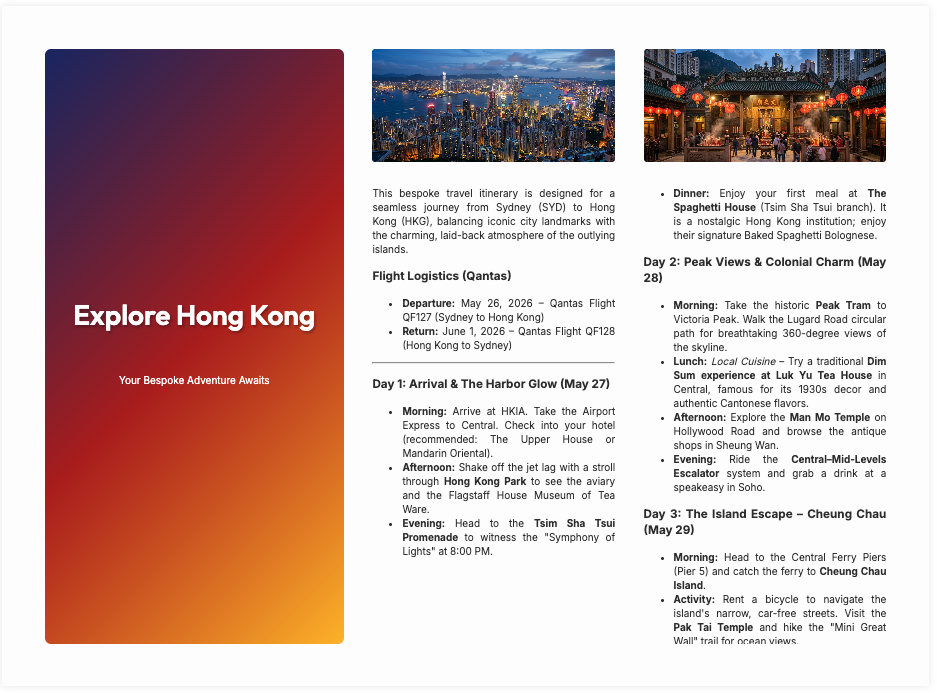
\includegraphics[keepaspectratio,alt={Page 1: Multi-modal travel pamphlet showcasing stateful orchestration and image generation.}]{figures/Itinerary Page 1.png}}
\caption{Page 1: Multi-modal travel pamphlet showcasing stateful
orchestration and image generation.}\label{fig:travel_workflow_a}
\end{figure}

\begin{figure}
\centering
\pandocbounded{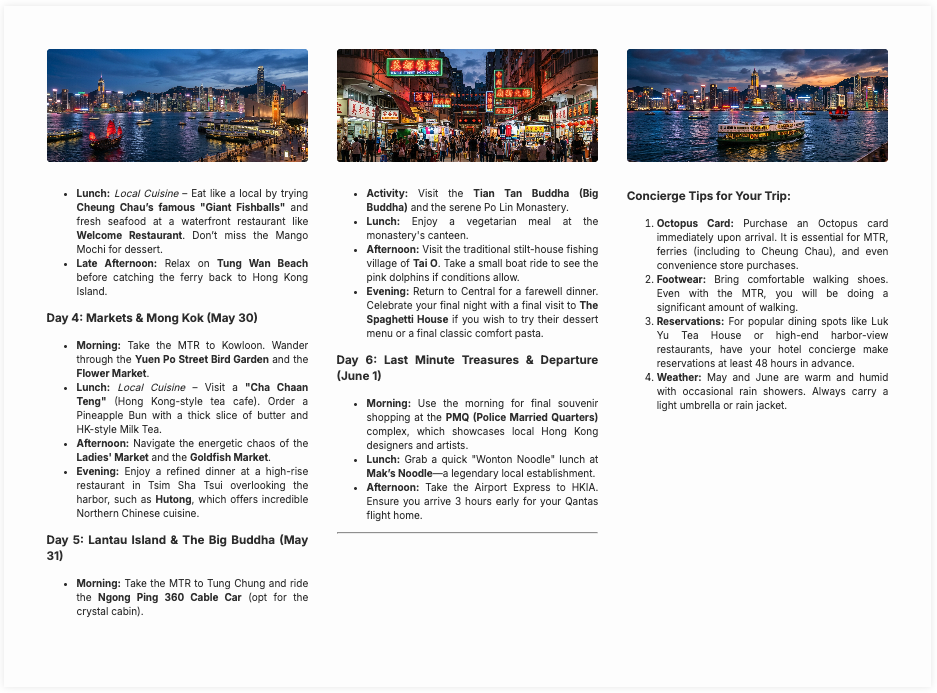
\includegraphics[keepaspectratio,alt={Page 2: Final formatted CSS-styled HTML itinerary.}]{figures/Itinerary Page 2.png}}
\caption{Page 2: Final formatted CSS-styled HTML
itinerary.}\label{fig:travel_workflow_b}
\end{figure}

Generated Multi-modal travel pamphlet for a Sydney to Hong Kong
itinerary.

\subsubsection{Declarative Workflow
Excerpt}\label{declarative-workflow-excerpt}

\begin{Shaded}
\begin{Highlighting}[]
\FunctionTok{graph}\KeywordTok{: }\CharTok{|}
\NormalTok{  graph LR}
\NormalTok{    Planner["Travel Planner | type=llm | role\_id=travel\_concierge"]}
\NormalTok{    Validator["Constraint Auditor | type=logic | logic\_id=validate\_constraints"]}
\NormalTok{    ImageGate["Image Gate | type=logic | logic\_id=check\_image\_status"]}
\NormalTok{    ImageGenerator["Image Generator | type=logic | logic\_id=generate\_and\_save\_images"]}
\NormalTok{    TemplateManager["Template Provider | type=logic | logic\_id=provide\_template"]}
\NormalTok{    PamphletFormatter["Pamphlet Formatter | type=logic | logic\_id=format\_pamphlet"]}
\NormalTok{    Finalizer["Itinerary Saver | type=logic | logic\_id=save\_itinerary"]}

\NormalTok{    Planner {-}{-}\textgreater{} Validator}
\NormalTok{    Validator {-}{-} "fail" {-}{-}\textgreater{} Planner}
\NormalTok{    Validator {-}{-} "pass" {-}{-}\textgreater{} ImageGate}
\NormalTok{    ImageGate {-}{-}\textgreater{} ImageGenerator}
\NormalTok{    ImageGate {-}{-}\textgreater{} TemplateManager}
\NormalTok{    ImageGenerator {-}{-}\textgreater{} TemplateManager}
\NormalTok{    TemplateManager {-}{-}\textgreater{} PamphletFormatter}
\NormalTok{    PamphletFormatter {-}{-}\textgreater{} Finalizer}

\FunctionTok{roles}\KeywordTok{:}
\FunctionTok{  travel\_concierge}\KeywordTok{: }\CharTok{\textgreater{}}
\NormalTok{    You are a professional travel concierge...}
\end{Highlighting}
\end{Shaded}

\begin{figure}
\centering
\pandocbounded{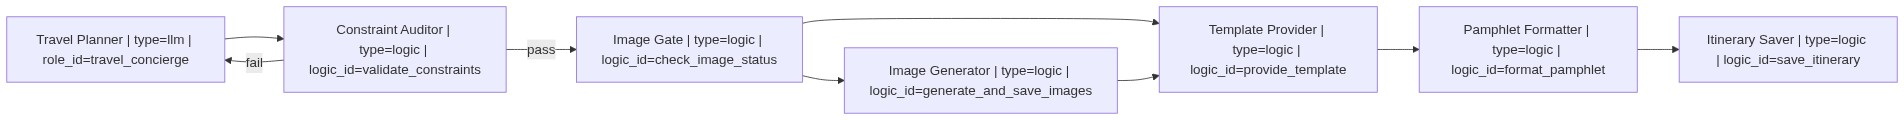
\includegraphics[keepaspectratio,alt={Visual DAG structure of the multi-modal travel itinerary planner, featuring iterative validation loops and parallel generation paths.}]{figures/travel_workflow.png}}
\caption{Visual DAG structure of the multi-modal travel itinerary
planner, featuring iterative validation loops and parallel generation
paths.}\label{fig:travel_graph}
\end{figure}

\subsubsection{R Orchestration (Minimal)}\label{r-orchestration-minimal}

\begin{Shaded}
\begin{Highlighting}[]
\FunctionTok{library}\NormalTok{(HydraR)}
\NormalTok{wf }\OtherTok{\textless{}{-}} \FunctionTok{load\_workflow}\NormalTok{(}\StringTok{"hong\_kong\_travel.yml"}\NormalTok{)}
\NormalTok{dag }\OtherTok{\textless{}{-}} \FunctionTok{spawn\_dag}\NormalTok{(wf, }\FunctionTok{auto\_node\_factory}\NormalTok{())}
\NormalTok{results }\OtherTok{\textless{}{-}}\NormalTok{ dag}\SpecialCharTok{$}\FunctionTok{run}\NormalTok{(}\AttributeTok{initial\_state =}\NormalTok{ wf}\SpecialCharTok{$}\NormalTok{initial\_state)}
\end{Highlighting}
\end{Shaded}

\subsection{Parallel Sorting Algorithm
Comparison}\label{parallel-sorting-algorithm-comparison}

This benchmarking example tasks three distinct LLM agents with
simultaneously implementing different sorting algorithms.
\texttt{HydraR} executes each task within an isolated
\texttt{Git\ worktree} to aggressively uncouple filesystem side-effects
and prevent merge conflicts. Following execution, a Merge Harmonizer
noded systematically reconciles the independent branches back to the
main state, preceding a terminal logic node that empirically benchmarks
the aggregated algorithms across five continuous trials
(\autoref{fig:sorting}).

\begin{figure}
\centering
\pandocbounded{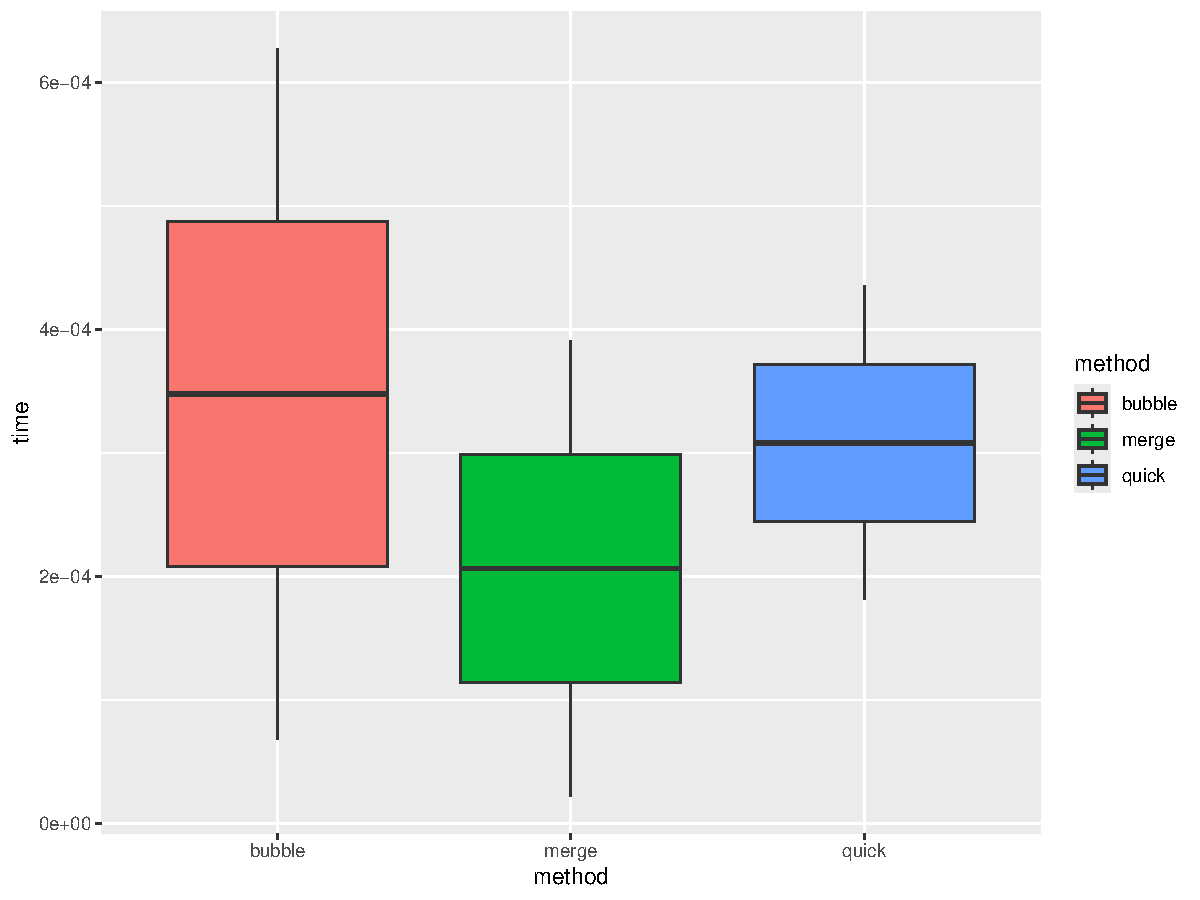
\includegraphics[keepaspectratio,alt={Sorting Algorithm Performance Benchmark (1,000 elements over 5 trials).}]{figures/sorting_benchmark.pdf}}
\caption{Sorting Algorithm Performance Benchmark (1,000 elements over 5
trials).}\label{fig:sorting}
\end{figure}

\subsubsection{Declarative Workflow
Excerpt}\label{declarative-workflow-excerpt-1}

\begin{Shaded}
\begin{Highlighting}[]
\FunctionTok{graph}\KeywordTok{: }\CharTok{|}
\NormalTok{  graph LR}
\NormalTok{      bubble["Bubble Agent | type=llm | role\_id=bubble"]}
\NormalTok{      quick["Quick Agent | type=llm | role\_id=quick"]}
\NormalTok{      merge["Merge Agent | type=llm | role\_id=merge"]}
\NormalTok{      merger["Merge Harmonizer | type=merge"]}
\NormalTok{      benchmark["Benchmark | type=logic | logic\_id=run\_benchmark"]}

\NormalTok{      bubble {-}{-}\textgreater{} merger}
\NormalTok{      quick {-}{-}\textgreater{} merger}
\NormalTok{      merge {-}{-}\textgreater{} merger}
\NormalTok{      merger {-}{-}\textgreater{} benchmark}
\end{Highlighting}
\end{Shaded}

\begin{figure}
\centering
\pandocbounded{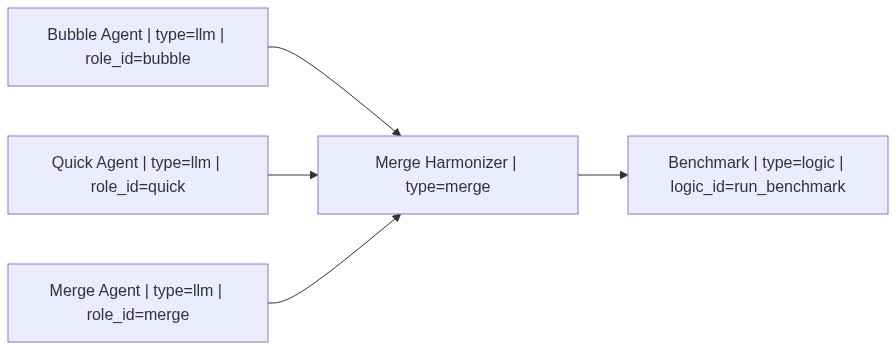
\includegraphics[keepaspectratio,alt={Visual representation of the parallel sorting comparison workflow, showing the fan-out/fan-in pattern and the merge harmonizer.}]{figures/sorting_workflow.png}}
\caption{Visual representation of the parallel sorting comparison
workflow, showing the fan-out/fan-in pattern and the merge
harmonizer.}\label{fig:sorting_graph}
\end{figure}

\subsubsection{R Orchestration (Parallel with
Isolation)}\label{r-orchestration-parallel-with-isolation}

\begin{Shaded}
\begin{Highlighting}[]
\FunctionTok{library}\NormalTok{(HydraR)}
\NormalTok{wf }\OtherTok{\textless{}{-}} \FunctionTok{load\_workflow}\NormalTok{(}\StringTok{"sorting\_benchmark.yml"}\NormalTok{)}
\NormalTok{dag }\OtherTok{\textless{}{-}} \FunctionTok{spawn\_dag}\NormalTok{(wf, }\FunctionTok{auto\_node\_factory}\NormalTok{())}
\NormalTok{results }\OtherTok{\textless{}{-}}\NormalTok{ dag}\SpecialCharTok{$}\FunctionTok{run}\NormalTok{(}\AttributeTok{initial\_state =}\NormalTok{ wf}\SpecialCharTok{$}\NormalTok{initial\_state, }\AttributeTok{use\_worktrees =} \ConstantTok{TRUE}\NormalTok{)}
\end{Highlighting}
\end{Shaded}

\subsection{Fault-Tolerant Pipelines with DuckDB
Persistence}\label{fault-tolerant-pipelines-with-duckdb-persistence}

To mitigate transient failures inherent to long-running scientific
workflows, \texttt{HydraR} integrates advanced checkpoint-and-resume
functionality powered by DuckDB (Raasveldt and Mühleisen 2019). Whenever
a pipeline pauses mid-execution, it automatically persists its complete
\texttt{AgentState}. Upon restart, any operator-applied programmatic
interventions are seamlessly merged, actively preventing redundant
evaluations by allowing execution to jump directly back to the paused
node.

\subsubsection{Declarative Workflow
Definition}\label{declarative-workflow-definition}

\begin{Shaded}
\begin{Highlighting}[]
\FunctionTok{graph}\KeywordTok{: }\CharTok{|}
\NormalTok{  graph LR}
\NormalTok{    Step1["Initialization"] {-}{-}\textgreater{} Step2["Risky Logic"]}
\NormalTok{    Step2["Risky Logic"] {-}{-}\textgreater{} Step3["Conclusion"]}
\FunctionTok{logic}\KeywordTok{:}
\FunctionTok{  check\_fixed}\KeywordTok{: }\CharTok{|}
\NormalTok{    if (!isTRUE(state$get("fixed"))) }
\NormalTok{      return(list(status = "PAUSE", output = "Waiting for manual fix."))}
\NormalTok{    list(status = "SUCCESS", output = "System recovered!")}
\end{Highlighting}
\end{Shaded}

\begin{figure}
\centering
\pandocbounded{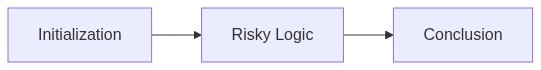
\includegraphics[keepaspectratio,alt={Visual logic of the fault-tolerant pipeline with DuckDB persistence, illustrating a linear flow with restartable checkpoints.}]{figures/fault_workflow.png}}
\caption{Visual logic of the fault-tolerant pipeline with DuckDB
persistence, illustrating a linear flow with restartable
checkpoints.}\label{fig:fault_graph}
\end{figure}

\subsubsection{Checkpoint and Resume}\label{checkpoint-and-resume}

\begin{Shaded}
\begin{Highlighting}[]
\FunctionTok{library}\NormalTok{(HydraR)}
\NormalTok{wf    }\OtherTok{\textless{}{-}} \FunctionTok{load\_workflow}\NormalTok{(}\StringTok{"state\_persistence.yml"}\NormalTok{)}
\NormalTok{dag   }\OtherTok{\textless{}{-}} \FunctionTok{spawn\_dag}\NormalTok{(wf)}
\NormalTok{saver }\OtherTok{\textless{}{-}}\NormalTok{ DuckDBSaver}\SpecialCharTok{$}\FunctionTok{new}\NormalTok{(}\AttributeTok{db\_path =} \StringTok{"history.duckdb"}\NormalTok{)}
\NormalTok{tid   }\OtherTok{\textless{}{-}} \StringTok{"reprex{-}session{-}001"}

\CommentTok{\# Run 1: Pauses at Step2 — state saved to DuckDB}
\NormalTok{res1 }\OtherTok{\textless{}{-}}\NormalTok{ dag}\SpecialCharTok{$}\FunctionTok{run}\NormalTok{(}\AttributeTok{thread\_id =}\NormalTok{ tid, }\AttributeTok{checkpointer =}\NormalTok{ saver,}
                \AttributeTok{initial\_state =} \FunctionTok{list}\NormalTok{(}\AttributeTok{fixed =} \ConstantTok{FALSE}\NormalTok{))}

\CommentTok{\# Run 2: Fix applied, resume from Step2}
\NormalTok{res2 }\OtherTok{\textless{}{-}}\NormalTok{ dag}\SpecialCharTok{$}\FunctionTok{run}\NormalTok{(}\AttributeTok{thread\_id =}\NormalTok{ tid, }\AttributeTok{checkpointer =}\NormalTok{ saver,}
                \AttributeTok{initial\_state =} \FunctionTok{list}\NormalTok{(}\AttributeTok{fixed =} \ConstantTok{TRUE}\NormalTok{),}
                \AttributeTok{resume\_from =} \StringTok{"Step2"}\NormalTok{)}
\end{Highlighting}
\end{Shaded}

By safeguarding computational progress autonomously, this pattern
effectively circumvents prohibitively costly re-execution in data
science pipelines reliant on voluminous LLM invocations or laborious
large-scale database queries.

\section{Research Impact Statement}\label{research-impact-statement}

\texttt{HydraR} is actively deployed at the \textbf{Australian Proteome
Analysis Facility (APAF)} to architect and automate resilient
bioinformatics tooling. Its declarative YAML schemas empower
non-programming domain experts to routinely govern advanced LLM logic
pipelines without any R coding proficiency, thereby democratizing the
scale and reproducibility of model-assisted scientific research.

\section{AI Usage Disclosure}\label{ai-usage-disclosure}

Transparency and accountability are core tenets of the \texttt{HydraR}
paradigm. A substantial portion of the implementation was co-developed
utilizing \textbf{Antigravity}, an agentic AI coding assistant,
supervised by a rigorous ``human-in-the-loop'' review protocol.
Specifically, the original authors independently conceptualized the
underlying system architecture, while the AI generated specialized
logic, unit tests, and software documentation with every resultant
commit sequentially tested and manually verified.

\section{Acknowledgements}\label{acknowledgements}

We acknowledge funding from \textbf{Bioplatforms Australia}, enabled by
the \textbf{National Collaborative Research Infrastructure Strategy
(NCRIS)}.

\section*{References}\label{references}
\addcontentsline{toc}{section}{References}

\protect\phantomsection\label{refs}
\begin{CSLReferences}{1}{1}
\bibitem[\citeproctext]{ref-R6}
Chang, Winston. 2021. \emph{R6: Recursive Object-Oriented Class System}.
\url{https://R6.r-lib.org}.

\bibitem[\citeproctext]{ref-langchain}
Chase, Harrison. 2022. {``LangChain: Building Applications with LLMs
Through Composability.''} \emph{GitHub Repository}.
\url{https://github.com/langchain-ai/langchain}.

\bibitem[\citeproctext]{ref-mall}
Couch, Simon P. 2024. \emph{Mall: Run Language Models Multiple Times}.
\url{https://github.com/simonpcouch/mall}.

\bibitem[\citeproctext]{ref-igraph}
Csárdi, Gábor, and Tamás Nepusz. 2006. {``The Igraph Software Package
for Complex Network Research.''} \emph{InterJournal} Complex Systems:
1695. \url{https://igraph.org}.

\bibitem[\citeproctext]{ref-google2025gemini}
Google. 2025. \emph{Gemini 1.5 Flash}.
\href{https://gemini.google.com}{Https://gemini.google.com}.

\bibitem[\citeproctext]{ref-crewai}
Moura, João. 2023. {``CrewAI: Collaborative AI Agents.''} \emph{GitHub
Repository}. \url{https://github.com/joaomoura/crewai}.

\bibitem[\citeproctext]{ref-gptstudio}
Nivard, Michel, and James Wade. 2024. \emph{Gptstudio: Use Large
Language Models Directly in Your Development Environment}.
\url{https://github.com/MichelNivard/gptstudio}.

\bibitem[\citeproctext]{ref-duckdb}
Raasveldt, Mark, and Hannes Mühleisen. 2019. {``DuckDB: An Embeddable
Analytical Database.''} \emph{Proceedings of the 2019 International
Conference on Management of Data (SIGMOD)}, ahead of print.
\url{https://doi.org/10.1145/3299869.3320212}.

\bibitem[\citeproctext]{ref-reticulate}
Ushey, Kevin, JJ Allaire, and Yuan Tang. 2024. \emph{Reticulate:
Interface to 'Python'}. \url{https://rstudio.github.io/reticulate/}.

\bibitem[\citeproctext]{ref-furrr}
Vaughan, Davis, and Dan Reznik. 2022. \emph{Furrr: Apply Mapping
Functions in Parallel Using Futures}.
\url{https://github.com/DavisVaughan/furrr}.

\bibitem[\citeproctext]{ref-ellmer}
Wickham, Hadley, Joe Cheng, Aaron Jacobs, Garrick Aden-Buie, and Barret
Schloerke. 2025. \emph{Ellmer: Chat with Large Language Models}.
\url{https://ellmer.tidyverse.org}.

\end{CSLReferences}

\end{document}
